\documentclass[hidelinks, 12pt, oneside]{article}
\usepackage{graphicx}
\usepackage{bookmark}
\usepackage{hyperref}
\usepackage{epsfig}
\usepackage{epstopdf}
\usepackage{caption}


%\graphicspath{{}}
\begin{document}
 
%titlepage
\thispagestyle{empty}
\begin{center}
\begin{minipage}{0.75\linewidth}
    \centering
%University logo
    
\includegraphics[width=13cm]{./graphics/universityLogo.jpg}
    \rule{0\linewidth}{0.15\linewidth}\par

%Thesis title
    {\uppercase{\Large Project Storm \par}}
   	{\uppercase{\Large Team NAME \par}}
    \vspace{1cm}
%Author's name
    {\normalsize Renaldo van Dyk 12204359\par}
    {\normalsize Andreas du Preez 12207871\par}
    {\normalsize Sean Hill 12221458\par}
    {\normalsize Shaun Meintjes 133310896\par}
    {\normalsize Johann Dian Marx 12105202\par}
    
    \vspace{1cm}
    
    \href{https://github.com/DianMarx/STORM}{GitHub link}
    \vspace{1cm}
	
\end{minipage}
\end{center}
\clearpage

\tableofcontents
\newpage
\section{Vision and Scope}
\subsection{History and Background}
\subsubsection{A Brief History of Project STORM}
In 2013 lecturers of the department of Computer Science, which resides at the University of Pretoria,
approached honors students of the module ``Educational Software Development'' to develop a team
shuffling system. 
The system was going to be used by the lecturers of the module ``Software Engineerin'' to
determine teams for the ``Rocking the boat'' exercise of the ``Software Engineering'' module using a
set of lecturer defined criteria to select the teams with. An incomplete requirements specification document
was designed and the project was brought to an end. 

\subsubsection{Project Background}
The lecturers of the ``Software Engineering'' module sought the need for such a shuffling tool, this
time approaching students of the ``Software Development'' module. The requirements specification previously 
developed will be used as a starting point. This document will be stripped down to a ``basic system'' requirements
specification, not completely discarding functionality specified in the previous documentation but adding relevant functionality
as the development life-cycle persists.

\subsection{Project Scope}
The complete system should enable users to build teams, from a list of students, by selecting a
set of criteria. This will aid the users in such a way that the users do not have to build the teams
manually, which may require a lot of time. The users can spend their time rather on analyzing
the results of each ``Rocking the Boat'' round to change the criteria for the next round more
effectively.


\section{Application requirements and design}
\subsection{Modular Design}


\begin{flushleft}
The system is to be a modular system which allows for:
\end{flushleft}

\begin{itemize} 
\item[$\bullet$] Only a subset of modules to be deployed. Minimally the system will require the core modules to be deployed.
\item[$\bullet$] Further modules to be added at a later stage.
\end{itemize}

\begin{flushleft}
To this end there should be:
\end{flushleft}

\begin{itemize} 
\item[$\bullet$] Minimal dependencies between modules, and
\item[$\bullet$] No dependencies of core modules on any add-on modules.
\end{itemize}

\begin{flushleft}
Modular design allows that each module encapsulates information that is not available to the rest of the program. This information hiding reduces the cost of subsequent design changes when future functionality is added to STORM. For example, if at a later stage functionality is added to allow for personality tests to be completed within STORM and results are automatically pulled in, a new module can be added without affecting other modules.
\end{flushleft}

\begin{figure}[h]
\centering
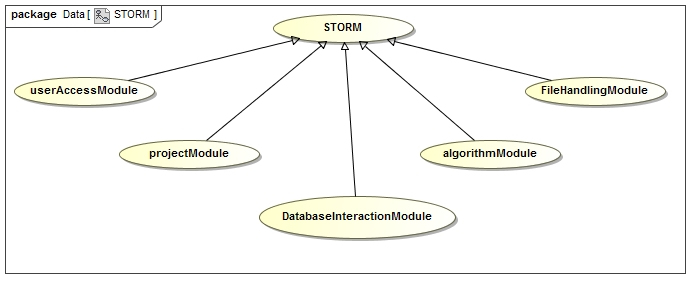
\includegraphics[width=15cm]{./graphics/stormOverview.jpg}
\caption{High level overview of STORM}
\end{figure}
\subsection{User Access Module}
This module deals with the STORM user access, specifically signing up, logging in, logging out and user authentication.

\subsubsection{Use-cases}
\begin{figure}[H]
    \centering
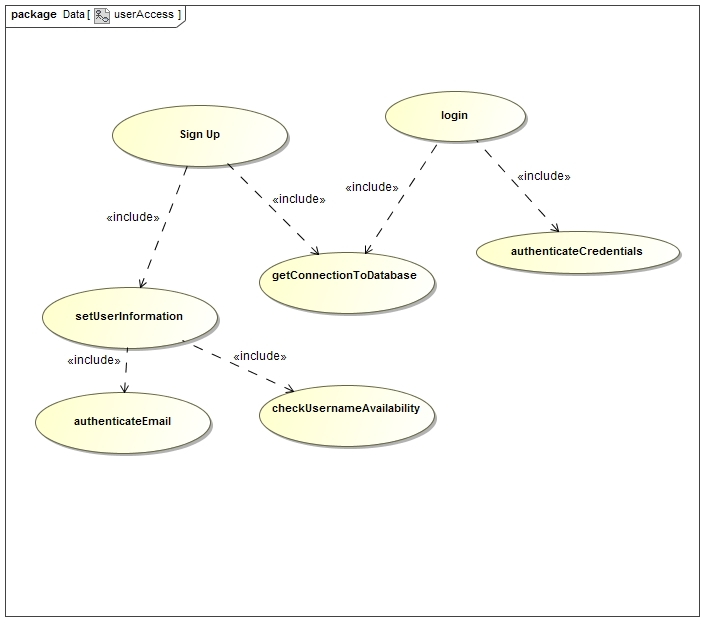
\includegraphics[width=15cm]{./graphics/userAccessUseCase.jpg}
    \caption{ User access module use case}
\end{figure}

    \rule{0\linewidth}{0.15\linewidth}\par
\begin{enumerate}
\item Sign Up\par
Priority: Critical.\par
Pre-condition: Client must have a valid e-mail address.\par
Post-condition: Client has a STORM profile.\par
\begin{figure}[H]
    \centering
    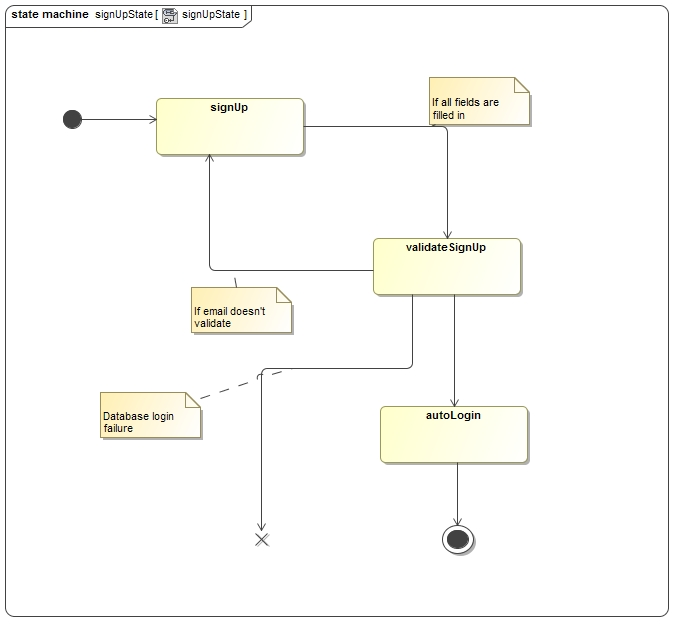
\includegraphics[width=15cm]{./graphics/signUpState.jpg}
    \caption{SignUp state diagram}
\end{figure}
\item Login\par
Priority: Critical.\par
Pre-condition: Client must have a STORM profile.\par
Post-condition: Client can now use STORM functionality.\par
\item Log out\par
Priority: Critical.\par
Pre-condition: Client must be logged into STORM.\par
\begin{figure}[H]
    \centering
    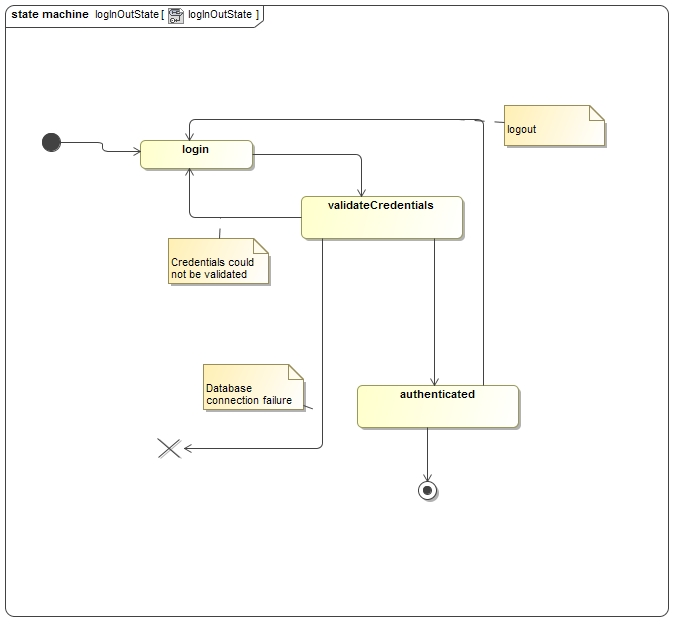
\includegraphics[width=15cm]{./graphics/logInOutState.jpg}
    \caption{Login/logout state diagram}
\end{figure}
\end{enumerate}


\subsection{Project Module}
This module deals with the configuration of projects. Initially a skeleton project will be set up with basic criteria 
and additional criteria can be added at a later stage as needed.
\subsubsection{Use-cases}
The projects mojule provides services create and manipulate projects.\par
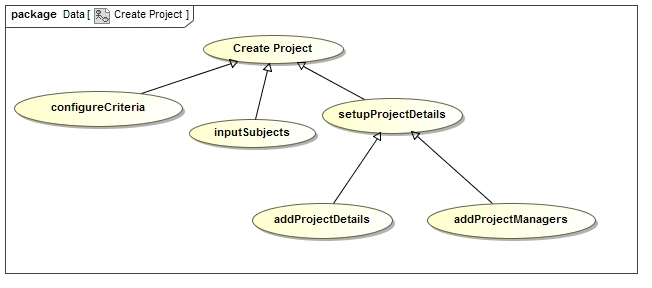
\includegraphics[width=13cm]{./graphics/createProjectUseCase.jpg}
    \rule{0\linewidth}{0.15\linewidth}\par
\begin{enumerate}
\item addProjectDetails\par
Priority: Critical.\par
Pre-condition: Client must be logged in.\par
Post-condition: Client must have a STORM profile.\par
Post-condition: Project skeleton is created in database.\par
\item addProjectManagers\par
Priority: Important.\par
Pre-condition: Client must have a STORM profile.\par
Pre-condition: Manager to be added must have a STORM profile.\par
Pre-condition: Client must have created a STORM project.\par
Post-condition: Manager has permition to colaborate on the project.\par
\item inputSubjects\par
Priority: Critical.\par
Pre-condition: Client must have a STORM profile.\par
Pre-condition: Client must have created a STORM project skeleton.\par
Post-condition: Project database is updated with a list of subjects.\par
\item ConfigureCriteria\par
Priority: Critical.\par
Pre-condition: Client must have a STORM profile.\par
Pre-condition: Client must be logged into STORM.\par
Pre-condition: Client must have created a STORM project skeleton.\par
Post-condition: Criteria for project is changed.\par
\end{enumerate}
\begin{figure}[h]
    \centering
    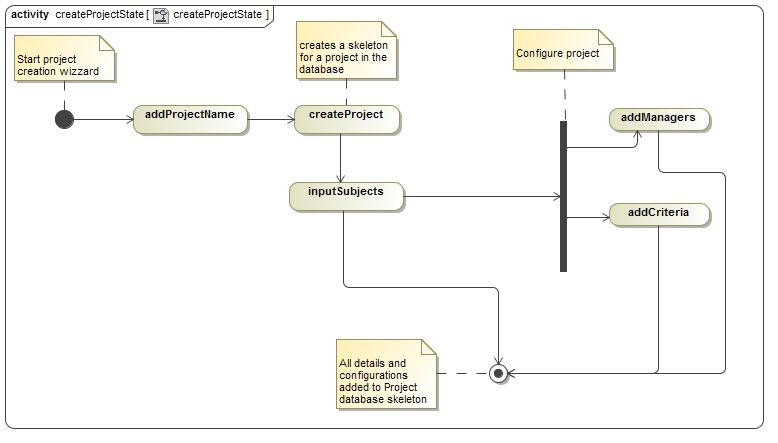
\includegraphics[width=15cm]{./graphics/createProjectState.jpg}
    \caption{createProject sate diagram}
    \label{fig:createProject_state}
\end{figure}
\subsection{Database Interaction Module}
include use cases here
\subsection{Algorithm Module}
This module deals with the main process behind STORM, it is the shuffling algorithm.

\subsubsection{Use-cases}
The algorithm module adds the functionality required to shuffle subjects into teams.\par
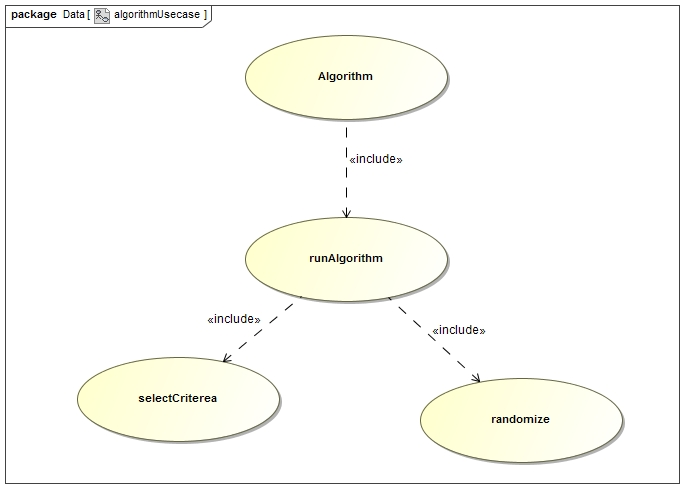
\includegraphics[width=13cm]{./graphics/algorithmUsecase.jpg}
    \rule{0\linewidth}{0.15\linewidth}\par

\begin{enumerate}
\item Randomize\par
Priority: Critical.\par
Pre-condition: Project must have users.\par
Pre-condition: Team size or number of teams must be specified.\par
Post-condition: Random teams are built.\par
    \begin{figure}
        \centering
        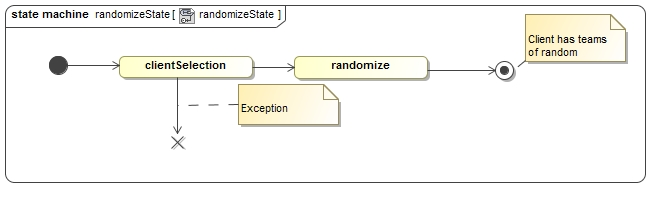
\includegraphics[width=13cm]{./graphics/randomizeState.jpg}
        \caption{Randomize state diagram}
        \label{fig:randomize_state}
    \end{figure}
\end{enumerate}
To be completed in future iterations
\pagebreak
\subsection{Reporting Module}
To be completed in future iterations
\section{Architectural Requirements}
This section discusses the software architecture requirements — that is the requirements around the
software infrastructure within which the application functionality is to be developed. The purpose
of this infrastructure is to address the non-functional requirements. In particular, the architecture
requirements specify
\begin{itemize}
	\item the architectural responsibilities which need to be addressed,
	\item the access and integration requirements for the system,
	\item the quality requirements, and
	\item the architecture constraints specified by the client
\end{itemize}
\subsection{Access and Integration Requirements}
This section discusses
\begin {enumerate}
\item the requirements for the different channels through which the system can be accessed by
people and systems, and
\item the integration channels which must be supported by this system.
This section specifies the different channels through which users will be able to access the system
services.
\end{enumerate}
\subsubsection{Human Access Channels}
The system will be accessible by human users through the following channels:\par
\begin{itemize}
\item From a web browser through a rich web interface. The system must be accessible from any of the standards-compliant web browsers including all recent versions of Mozilla Firefox, Google Chrome, Apple Safari and Microsoft Internet Explorer.
\item From mobile devices if time allows it.
\end{itemize}
\subsubsection{System Access Channels}
\begin{itemize}
\item Other systems should be able to access services offered by STORM. Perhaps direct feed of teams into other systems.
\item Various technologies will be used such as:
	\begin{itemize}
	\item Node.js
	\item Express.js
	\item EJS
	\item Mongoose
	\item SMTP
	\end{itemize}
\end{itemize}
\subsubsection{Integration channels}
The system will allow manual integration through importing and exporting of CSV
files. In particular, the system will support
\begin{itemize}
\item Importing of subject data from CSV files.
\item Importing of new criteria for shuffling subjects from CSV files.
\item Exporting of groups to CSV files.
\item Exporting of subject data for offline editing to CSV files.
\end{itemize}



\subsection{Quality Requirements}
The quality requirements are the requirements around the quality attributes of the systems and
the services it provides. Quality requirements relevant to project STORM are listed below in order of priority. \par

\subsubsection{Usability}
Usability is one of the most important quality attributes. Usability tests should be performed to check whether:
\begin{itemize}
\item whether users find any aspects of the system cumbersome, non-intuitive or frustrating.
\item whether the user has a positive experience and finds the functionality easy to use and learn.
\end{itemize}

\subsubsection{Scalability}
The system must implement a very generic optimization algorithm in order to be used by different parties in different contexts. In addition to different environments the system should be able to optimize groups for an extremely large number of subjects.

\subsubsection{Performance}
\begin{itemize}
\item The optimization algorithm should be able to sort a maximum of 10 000 subjects into groups and respond within 5 seconds.
\item Reporting queries should respond within 15 seconds. \par
The above figures does not include network round trip which is outside the control of the system.
\end{itemize}

\subsubsection{Maintainability} 
Amongst the most important quality requirements for the system is maintainability which includes flexibility and extensibility. It should be easy to maintain the system in the future. To this end
\begin{itemize}
\item future developers should be able to easily understand the system,
\item the technologies chosen for the system and be reasonably expected to be available for a long time,
\item and developers should be able to easily and relatively quickly
\begin{itemize}
\item change aspects of the functionality the system provides, and
\item add new functionality to the system.
\end{itemize}
\end{itemize}

\subsubsection{Reliability}
The system should provide by default a reasonable level of reliability and should be deployable within configurations which provide a high level availability, supporting
\begin{itemize}
\item fail-over safety of all components and
\item a deployment without single points of failure.
\end{itemize}
Hot deployment of new/changing functionality is not required for this system.

\subsubsection{Deployability}
The system must be deployable
\begin{itemize}
\item on Linux servers,
\item and in environments using different databases for persistence of the STORM data.
\end{itemize}

\subsubsection{Security}
\subsubsection{Testability}
All services offered by the system must be testable through
\begin{enumerate}
\item unit tests, testing components in isolation using mock objects, and
\item integration tests where components are integrated within the actual environment.
\end{enumerate}
In either case, these functional tests should verify that
\begin{itemize}
\item the service is provided if all pre-conditions are met (i.e. that no exception is raised except
if one of the pre-conditions for the service is not met), and
\item that all post-conditions hold true once the service has been provided.
\end{itemize}
In addition to functional testing, the quality requirements like scalability, usability, auditability,
performance and so on should also be tested.


\subsection{Architectural Responsibilities}
The architectural responsibilities for STORM includes the responsibilities of providing an infrastructure for
\begin{itemize}
\item a web access channel,
\item hosting and providing the execution environment for the services/business logic of the system,
\item persisting and providing access to domain objects,
\item logging,
\item and delivering reports readable by 3rd party applications.
\end{itemize}
\subsection{Architecture Constraints}
\begin{flushleft}The choice of architecture is largely unconstrained and the development team has the freedom to
choose the architecture and technologies best suited to fulfill the non-functional requirements for
the system subject to:
\end{flushleft}
\begin{enumerate}
\item The architecture being deployable on a server, such as the Linux server of the University of Pretoria.
\item The architecture is constrained to using web technology.
\end{enumerate}
\section{Architecture design}
\subsection{Overview}
MVC architecture - using express.js framework
\begin {enumerate}
\item Model - Database connection and access done via mongoose, requests handeled by AJAX.
\item View - ExpressJS defines a response object for rendering html views and serving the view with JSON data.
\item Controller - Defined in form of routes. ExpressJS routes  are middleware functions which accepts request and result objects used to route data.
\end {enumerate}
\subsection{Modularization}
The software architecture of STORM is a modular software architecture with a number of core modules
and a number of pluggable add-on modules. Further add-on modules can be added at a later stage.
Add-on modules may add additional functionality and may enrich excisting functionality through
interception.
\subsection{Architectural tactics addressing quality requirements}
This section discusses the architectural tactics which are used to concretely address the quality
requirements for the application

\subsubsection{Database abstraction}
The system includes a database abstraction module to improve:
\begin {itemize}
\item Deplayability as mentioned in section \ref {3.2.5} in environments where different databases are used,
\item Security as mentioned in section \ref {3.2.6} to isolate database and hide sesitive subject data.
\end {itemize}

\subsubsection{UI components framework}
The system will use a rich, dynamic JQuery-UI component library in order to:
\begin {itemize}
\item provide a rich, dynamic user interface for usability (requirement \ref {3.2.1}),
\item improve scalability (requirement \ref {3.2.2}) and performance (requirement \ref {3.2.3}).
\end{itemize}

\subsubsection{Maximize client-side scripting}
The system will use client-side javascript where possible to address:
\begin {itemize}
\item Performance (requirement \ref {3.2.3}) by avoiding the netork round trip,
\item scalability (requirement \ref {3.2.2}) and security (requirement \ref {3.2.6}) by hiding data out of a user's bounds.
\end{itemize}

\subsubsection{MVC}
The system will use a MVC pattern to address:
\begin {itemize}
\item Usability (requirement \ref {3.2.1}),
\item Deployability (requirement \ref {3.2.5}).
\end{itemize}

\end{document}
